\documentclass{report}

\usepackage[utf8]{inputenc} 		% Permet d'utiliser des sources LaTeX contenant des caractères accentués.
\usepackage[T1]{fontenc}				% Permet d'utiliser des sources LaTeX contenant des caractères accentués.
\usepackage[francais]{babel} 		% Permet de charger le package babel en lui indiquant que l'on veut travailler en français.
\usepackage[cyr]{aeguill} 			% Permet d'utiliser les guillemets français («»).
\usepackage{graphicx}           % Permet l'importation d'image.


\title{Améliorer la qualité des logiciels avec l'Intégration Continue}
\author{\textsc{Gaëtan Meynier}}
\date{\today}

\begin{document}

  \begin{titlepage}
    \centering
    {\scshape\LARGE Université Paris Dauphine \par}
    \vspace{1cm}
	  {\scshape\Large Mémoire de recherche\par}
    \vspace{0.5cm}
    Septembre 2016\par
    \vspace{4.5cm}
    {\huge\bfseries Améliorer la qualité des logiciels avec l'Intégration Continue\par}
    \vspace{2cm}
	  {\Large\itshape Gaëtan Meynier\par}
    \vspace{5cm}
	  \vfill
	    {\bfseries Supervisé par\par}
      \vspace{0.5cm}
	    Khalid \textsc{Belhajjame}, Maître de conférence à l'Université Paris Dauphine,
      Arthur \textsc{Szumovicz}, Consultant en système d'information à AXA.
	  \vfill
  \end{titlepage}

  \tableofcontents                % Table des matières.

  \chapter{Introduction}

    \section{Motivation}

    \section{Scope}

    \section{Problèmes de recherche}

    \section{Methodes}

      \subsection{Méthodes de recherche}

      \subsection{Collecte de données}

    \section{Structure du mémoire}

  \chapter{DevOps}

  \chapter{Intégration Continue}

    \section{Histoire}
    L'idée de l'Intégration Continue a été développée par la communauté Extreme Programming et a été décrit par Kent Beck dans son livre « Extreme programming explained » \cite{Bec99}. Martin Fowler a également été l'un des premiers contributeurs qui ont écrit sur l’intégration continue \cite{Fow00}. Plus tard, le travail a été poursuivi par Paul Duvall qui a écrit tout un livre à propos de l’intégration \cite{Duv07}.

    \section{L'Intégration Continue comme un processus}
    L’Intégration Continue est un processus où le logiciel est construit à chaque changement. Cela signifie que lorsqu’une modification apportée par un développeur est détectée dans le code source, une construction automatique est déclenchée sur une machine de construction séparé. La construction contient plusieurs étapes prédéfinies comme la compilation, les tests, la génération de métrique du code source et le déploiement - entre autres. Une fois la construction terminé un rapport est envoyé aux membres du projet spécifié. Le rapport de compilation indique le résultat de chaque étape de la construction avec des informations détaillées sur les erreurs possibles qui ont pu survenir.\\\\

    Martin Fowler \cite{Fow00} décrit l’Intégration Continue comme :\\
    \begin{quotation}
      \emph{« Continuous Integration is a software development practice where members of a team integrate their work frequently, usually each person integrates at least daily - leading to multiple integrations per day. Each integration is verified by an automated build (including test) to detect integration errors as quickly as possible. Many teams find that this approach leads to significantly reduced integration problems and allows a team to develop cohesive software more rapidly. »}
    \end{quotation}

    \begin{quotation}
      \emph{« L'Intégration Continue est une pratique de développement logiciels où les membres d'une équipe intègre leur travail régulièrement, chaque développeur intègre au moins quotidienne une version - conduisant à de multiples intégrations journalière. Chaque intégration est vérifiée par une construction automatique (y compris le test) pour détecter les erreurs d'intégration le plus rapidement possible. De nombreuses équipes trouvent que cette approche conduit à réduire considérablement les problèmes d'intégration et permet une équipe pour développer des logiciels cohésifs plus rapidement. »}\\
    \end{quotation}

      \subsection{Les bénéfices de l’Intégration Continue}
      Selon Paul Duvall \cite{Duv07}, l'intégration logiciels n’est pas un problème dans les petites équipe, un à deux développeurs, mais quand le nombre de collaborateur se multiplie ou que diverses équipes commencent à travailler ensemble sur un projet, l'intégration logiciels devient un problème, car plusieurs personnes modifient simultanément des morceaux de code devant fonctionner ensemble. Vérifier que les divers composants logiciels interdépendants continuent de fonctionner correctement ensemble soulève la nécessité d'intégrer plus tôt et plus souvent. Les points suivants décrivent les différents effets bénéfiques que Paul Duvall a été en mesure d'identifier.

        \subsubsection{Réduire les risques}
        En intégrant plusieurs fois par jour, les risques de dysfonctionnement sont considérablement réduits. Les problèmes sont remontés dès leur intégration et peuvent même être la cause d’un rejet d’intégration. Ceci étant possible par l’intégration et l’exécution de tests et l’inspections automatiquement du code source après chaque modification.

        \subsubsection{Générer des logiciels déployables}
        L'un des objectifs du développement logiciel agile est de déployer tôt et souvent. L’Intégration Continue aide à atteindre cet objectif en automatisant les étapes de production des logiciels déployables. Des logiciels déployables et fonctionnels est l'avantage le plus évident de l’Intégration Continue du point de vue extérieur, car le client ou l'utilisateur final est généralement pas intéressés par le fait que l’Intégration Continue ait été utilisé dans le cadre de l'assurance qualité. Il est aussi l'atout le plus tangible, étant le résultat final de l’Intégration Continue.

        \subsubsection{Permettre une meilleure visibilité du projet}
        Le fait que le processus d’Intégration Continue s’exécute régulièrement fournit la capacité à remarquer les tendances et à prendre des décisions sur la base d’informations réelles. Sans Intégration Continue, les informations doivent être recueillies manuellement requérant du temps et des efforts. Le  processus d’Intégration Continue fourni en temps réel les informations sur l'état de la construction et de la qualité des dernières mesures tels que la couverture de test ou le nombre de codage violations de la convention.

        \subsubsection{Une plus grande confiance du produit}
        En ayant une Intégration Continue en place, l'équipe projet se protège contre certaines actions négatives portées aux codes sources. L’Intégration Continue agit comme un filet de sécurité, il repère les erreurs tôt et régulièrement. Ce qui se traduit par une plus grande confiance à l'équipe. Même des changements importants peuvent être faits avec confiance.

      \subsection{Le cycle de travail de l’Intégration Continue}
      Alors que l’Intégration Continue est généralement orchestrée par un serveur d’Intégration Continue, c’est aussi une façon de travailler. L'idée principale est d'intégrer les changements au code source aussi souvent qu’il y ait du nouveau code ajoutant de la valeur à l’application, à savoir plusieurs fois par jour. Cela rend l'intégration du code plus facile parce qu'il y a moins de code à intégrer à la fois. Il contribue également dans une situation où plusieurs personnes modifient la même base de code, car les développeurs auront ainsi les modifications apportées par d'autres.
      L'intégration des changements au code source de base comporte plusieurs étapes. Le cycle de travail est illustré dans le schéma suivant (Voir Figure \ref{IC workflow}). Il est basé sur les idées présentées par Martin Fowler \cite{Fow00} avec une phase de mise à jour supplémentaire, après l'exécution des tests. Cette phase de mise à jour est nécessaire dans la situation où le test prend du temps de sorte qu'il pourrait déjà y avoir de nouvelles modifications intégrées pendant notre phase de test.\\

      \begin{enumerate}
        \item récupérer le code source du référentiel (Check-out),
        \item modifier le code et créer les tests pour les modifications,
        \item vérifiez si quelqu'un d'autre a modifié le code source,
        \item exécuter tous les tests afin de vérifier que les modifications n’aient pas altéré le bon fonctionnement de l’application,
        \item vérifiez à nouveau si quelqu'un d'autre ont modifié le code source,
        \item valider les modifications dans le référentiel (Check-in),
        \item démarrer un nouveau cycle.\\
      \end{enumerate}

      \begin{figure}
        \begin{center}
          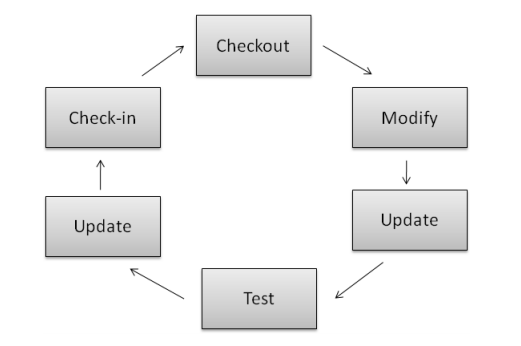
\includegraphics[scale=0.5]{images/ICWorkflow.png}
        \end{center}
        \caption{Cycle de travail de l’Intégration Continue}
        \label{IC workflow}
      \end{figure}

      Le cycle de travail commence créer une copie du code source hébergé sur le serveur de gestion de code qui est sur le point d'être modifié. Si le code avait précédemment récupéré, une mise à jour est faite à la place. Le développeur effectue les changements appropriés à sa tâche (nouvelle fonctionnalité, réfactorisation du code…) et implémente les tests appropriés afin de vérifier la conformité de son développement. Un test de développement vérifie que la sortie d’une méthode, en fonction de ses entrées, soit en adéquation avec le résultat attendu. Il est recommandé d’écrire les tests avant le code réel de l’application, ceci est appelé Test Driven Development (TDD).\\

      Dans un projet de logiciel, il est courant que de nombreux développeurs travaillent simultanément sur une même partie de code.  Par conséquent avant d’intégrer notre partie en code source, il est nécessaire de vérifier qu’aucune modification n’ait été faite par un développeur tierce sur par le biais d’une nouvelle mise à jour. Dans certains cas, il est possible que d’autres développeurs aient modifié exactement les mêmes lignes de code que nous produisant un ou plusieurs conflits. Dans ce cas, les conflits doivent être immédiatement résolus et tous les tests ré-effectués. Il est possible que dans cet intervalle une nouvelle version soit disponible sur le référentiel,  l'étape précédente doit être répétée jusqu'à ce qu'aucuns nouveaux changements ne soient détectés. Une fois cette synchronisation effectué le check-in peut être fait.

      \subsection{Comment l’Intégration Continue s’appuie-t-elle sur d’autres pratiques de développement}
      L’Intégration Continue comprend un ensemble de règles qui tous développeurs devraient suivre :

      \begin{enumerate}
        \item effectuer régulièrement des commits,
        \item ne pas commit des codes buggés,
        \item régler les problèmes et builder immédiatement,
        \item écrire des tests de développement automatisés,
        \item tous les tests et métriques doivent être valides,
        \item exécuter en local ses builds,
        \item éviter de travailler avec du code buggés.\\
      \end{enumerate}

      Ces règles ne sont pas nouvelles dans le monde du développement logiciel et sont aussi adopté d'autres pratiques de développement. Par conséquent, si des pratiques telles que les tests de développeur, les normes de codage, le refactoring et la propriété collective sont déjà mises en place au sein du projet, il est facile de commencer à utiliser l’Intégration Continue. Ces pratiques doivent être rigoureusement appliquées au travers de l’Intégration Continue sous peine d’empêcher les autres collaborateurs du projet de travailler. Prenons par exemple le cas d’un développeur ayant remanié une partie du code source et cassé quelques tests. Ne l’ayant pas remarqué, faute de n’avoir pas exécuté les tests, il valide ses changements dans le référentiel. La build éclate du faite que la règle « tous les tests doivent être au vert » n’est pas suivie. Maintenant si un autre développeur commence à travailler avec le code du référentiel, la première chose qu'il doit faire est de fixer ce qui avait été cassé par son collègue. Et cela peut prendre un beaucoup de temps, si cette personne ne connaît pas la partie de code qui provoque l’échec des tests.

    \section{L’Intégration Continue est un mélange de personnes et de systèmes}

      \subsection{Le développeur}
      !!!!!!!!!!!!!!!!! You build it, you run it !!!!!!!!!!!!!!!!!

      Pratiquer l’Intégration Continue exige de la discipline de la part des développeurs. Ils devront appliquer avec rigueur les pratiques de développement vus précédemment. Une fois le développement de la tâche effectué, le développeur doit exécuter une build sur sa propre machine de développement. On appelle cela une build privée. Cette étape permet de vérifier que les modifications apportées n’ont pas endommagé l'intégration avec le reste du code source. Il est important d'exécuter la build privée avant de valider les changements dans le référentiel de contrôle de version, car soumettre un code cassé peut empêcher les autres développeurs de travailler. Une fois l’exécution de la build privée avec succès, le développeur peut valider les modifications, et les tests. Si l'intégration de la build échoue malgré ses précautions, réparer cette build est la priorité numéro un.

      \subsection{Le référentiel de contrôle de version}
      L'intégration continue ne peut pas se faire sans référentiel de contrôle de version. Le référentiel de contrôle de version, également connu sous le nom de gestionnaire de code source (SCM), est un système utilisé pour stocker le code source et d'autres aspects du logiciel (comme la documentation) de manière centralisée. Il assure également le suivi de l'historique des versions et modifications effectuées au cours du développement. Les développeurs de logiciels ont la possibilité de revenir à une version antérieure ou la révision d'un logiciel, ou de prendre connaissances des changements apportés sur toute révision donnée. Ce référentiel fournit un point d'accès unique au code source pour les développeurs et le système d’Intégration Continue. Il peut être constitué de différentes branches du logiciel stocké. Une branche peut être créée pour la réécriture majeure d’un morceau de code ou pour le prototypage d’une idée intéressante qui pourrait ne pas se retrouver dans le produit final. La build d’intégration est exécuté sur la branche principale du référentiel de contrôle de version \cite{Duv07}. « Master » est la branche de code source où la plupart de la mise au point a lieu. Certains systèmes de contrôle de version appellent cela aussi « tunk » ou « head ». La ligne principale se doit d’être toujours stable et la build d’intégration ne doit jamais échouée quand elle est intégrée au référentiel.

      \begin{figure}
        \begin{center}
          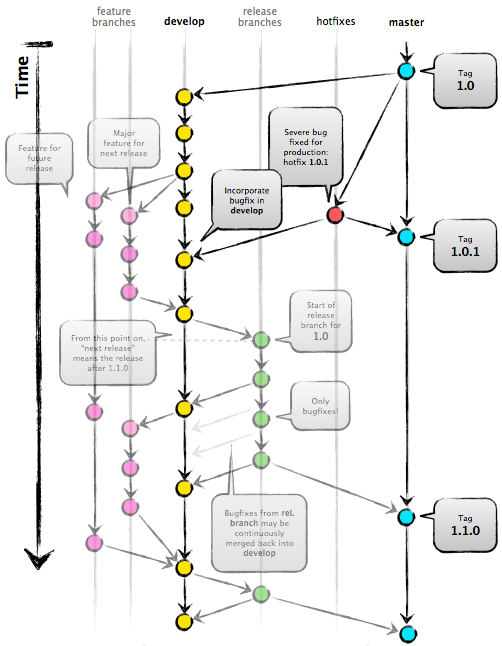
\includegraphics[scale=0.5]{images/gitFlow.png}
        \end{center}
        \caption{Ligne de temps d'un référentiel de contrôle de version}
      \end{figure}

      \subsection{Le serveur d’Intégration Continue}
      Le serveur d’Intégration Continue est l'orchestrateur de l'ensemble du processus. Il exécute la build d'intégration lorsqu'une modification a été apportée au référentiel. Quatre approches sont à prendre en compte.\\

      La première est la configuration d’un « post commit hook » au niveau du gestionnaire de code source. Le référentiel de contrôle de version peut-alors avertir immédiatement le serveur d’Intégration Continue qu’une modification a été ajoutée et validée. De cette façon une build d’intégration est exécutée pour chaque commit.\\

      Une autre approche, dénommée « polling approach »  \cite{Duv07} est de vérifier les changements à intervalles réguliers (de l’ordre de la minute). De ce fait plusieurs changements peuvent être effectués entre chaque build.\\

      Une troisième option est d’exécuter une build d’intégration à intervalles réguliers, mais si l'intervalle est trop long le bénéfice de la rétroaction est rapidement perdu.\\

      La quatrième et dernière option, consiste à intégrer une copie du référentiel principal, accessible uniquement par le serveur d’Intégration Continue, au niveau du serveur lui-même \ref{IC server}. Les développeurs n’ont ainsi accès qu’au référentiel du serveur d’Intégration Continue. Ce dernier peut alors être configuré afin de rejeter les modifications apporté au référentiel ne respectant pas les tests ou les métriques qualités prédéfinies. Garantissant ainsi la qualité de l’application.\\\\

      \begin{figure}
        \begin{center}
          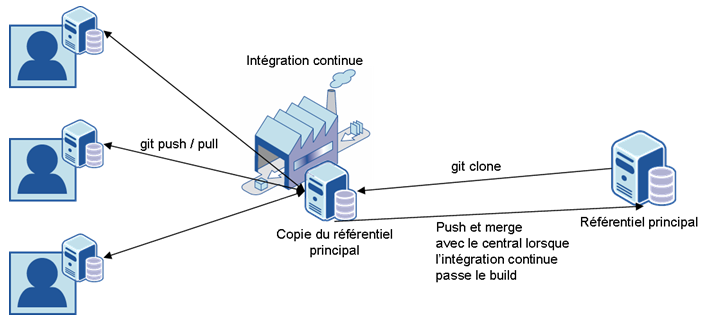
\includegraphics[scale=0.5]{images/ICServer.png}
        \end{center}
        \caption{Organisation d'un serveur d'Intégration Continue}
        \label{IC server}
      \end{figure}

      Le serveur d’Intégration Continue fournit également une vue, généralement une page web, qui expose l'état de santé de tous les « build jobs »\footnote{Build jobs : cela correspond aux différentes tâches du processus de build.} et afficher leurs résultats en temps réel  configurés (Voir Figure \ref{Jenkins build jobs}). Ce tableau de bord peut être affiché, par exemple, sur un grand écran dans la salle de l'équipe de développement pour donner un aperçu rapide et en temps réel des tâches effectués sur le serveur et voir ainsi s'il y a des constructions en cours d'exécution. De nombreux serveurs d’Intégration Continue proposent également un type de visualisation basé sur les principes des feux de circulation ou de météo de connaitre l’état des builds d’Intégration.\\

      Toutes les fonctionnalités d’un serveur d’Intégration Continue ne sont pas nécessaires pour faire de l’Intégration Continue. De nombreux scripts personnalisés peuvent effectuer les mêmes tâches, mais avoir un serveur conçu à cet effet aide beaucoup \cite{Duv07}. De plus en plus de solutions propriétaires ou open source\footnote{Open source : logiciel libre redistribution, d'accès au code source et de création de travaux dérivés.}  performe le marché et offre un environnement d’Intégration Continue stable et complet.\\

      Dans sa forme la plus simple, l’Intégration Continue pourrait être mise en place avec un seul ordinateur dédié exécutant des scripts afin de vérifier le code source du référentiel, lancer une build d’Intégration et envoyer des rapports une fois la build terminée. Le serveur d’Intégration Continue offre une autre possibilité en fournissant une interface utilisateur afin de configurer les multiples « build jobs ».

      \begin{figure}
        \begin{center}
          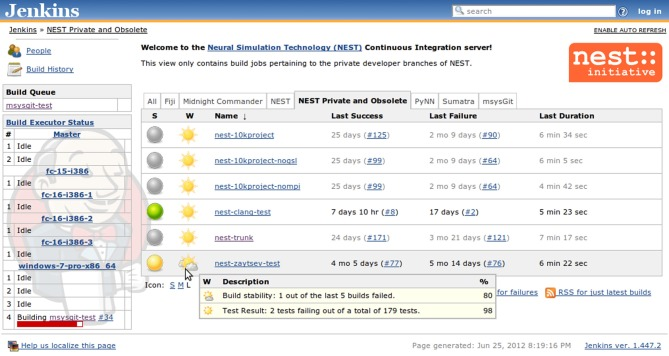
\includegraphics[scale=0.5]{images/jenkinsBuildJobs.png}
        \end{center}
        \caption{Tableau de bord d'un serveur d'Intégration Continue Jenkins}
        \label{Jenkins build jobs}
      \end{figure}

      \subsection{Les scripts de construction (build)}
      Généralement la plupart des étapes d’une build sont définies en utilisant un script de compilation. Un script de compilation peut être constitué d'un ou plusieurs scripts et il est utilisé, par exemple, pour compiler, tester, contrôler et déployer des logiciels. Toutes les mesures qui peuvent être automatisées pour construire et déployer des logiciels doivent être automatisées. Cela économise du temps et les nerfs des développeurs. Il existe de nombreuses techniques disponibles comme Ant (Java), Make (C/C++) ou Scons (Python).\\

      Certains développeurs utilisent leur environnement de développement intégré (IDE) pour builder leurs logiciels. Dans ce cas la build ne pourra être encadré par l’Intégration Continue. L’intégration Continue nécessite que la build puisse être exécutée indépendamment de tout IDE \cite{Duv07}.


      \subsection{Les mécanismes de feedback}
      Lorsque la build d'intégration est terminée, les résultats doivent être accessibles dès que possible. La capacité à fournir un feedback rapide est l'un des avantages de l’Intégration Continue. La rétroaction est disponible immédiatement une fois la build terminée. La rétroaction peut être diffusée par différent canaux ; tableau de bord, courrier électronique, flux RSS. En cas de build défectueuse, la réparation peut démarrer immédiatement après réception de l'avis.\\

      Certain pionnier commence même à intégrer le terme de « monitoring continue » dans l’ingénierie logicielle en complément de l’Intégration Continue. Le monitoring continu consiste à avoir un affichage visible par tous les membres de l’équipe de développement, actualisé en temps réel, donnant un feedback direct sur l’état des différentes builds simplifié et directement interprétable. Cet affichage est dans la plupart du temps un moniteur, mais d’autres solutions plus amusantes, telles que la lampe à lave ou une « ambient orb » commencent à s’imposer \cite{Swa04}.


      \subsection{Les machines de build d’intégration}
      Un serveur d’Intégration Continue à besoin d'un hôte pour fonctionner. La machine de build d’intégration (ou nœud)  est une machine distincte qui doit imiter l'environnement de production. Si possible, elle doit fonctionner avec le même système d'exploitation, la même version de serveur de base de données et les mêmes versions de librairies doivent être utilisées, comme il est prévu pour en production. Chaque différence augmente le risque des tests de ne pas détecter les problèmes liés à l’environnement de la production \cite{Fow06}.\\

      Dans le cas où de nombreux « build jobs » sont configurés pour l’application, pour réduire la durée de la build et ainsi augmenté la rapidité de la rétroaction il peut être nécessaire de paralléliser les tâches sur plusieurs machines (scalabilité horizontal). Certains logiciels de serveur d’Intégration Continue fournissent une architecture maître-esclave qui permet ainsi de diviser la charge de travail sur plusieurs hôtes.\\

      Parfois plusieurs environnements sont nécessaires pour builder sur différentes plates-formes. La virtualisation des serveurs apportent la réponse à ce problème. En utilisant une infrastructure de virtualisation bien établis, il est assez facile d’exécuter des instances esclaves multiples sur un seul nœud physique. Ces instances pouvant fonctionner sous différents systèmes d’exploitation. Certains logiciels de serveur d’Intégration Continue offre la possibilité à la build d’intégration de fonctionner simultanément sur ces différentes instances et de collecter les résultats pour chaque environnement.\\

      Puis virtualisation est quelque chose de valeur à l'aide de la peine de la virtualisation diminue \cite{Bar03}. Certains logiciels de serveur de CI comme Hudson permet même de construction de travail afin de fonctionner simultanément sur plusieurs serveurs virtuels et de collecter des résultats pour chaque environnement.


    \section{Caractéristique de l’Intégration Continue}
    Selon Paul Duvall \cite{Duv07} seules quatre caractéristiques sont nécessaires à l’Intégration Continue :\\
    \begin{itemize}
      \item une connexion à un référentiel de contrôle de version,
      \item un script de compilation,
      \item un mécanisme de rétroaction,
      \item un processus pour intégrer les modifications au code source (manuelles ou serveur d’Intégration Continue).\\
    \end{itemize}

    Ces éléments seuls sont nécessaires à la construction d’un système d’Intégration Continue efficace, qui est expliqué plus en détail dans les sections suivantes.


      \subsection{Compilation du code source}
      La compilation du code source est l'une des caractéristiques de base du système d’Intégration Continue. La compilation crée des exécutables binaires à partir de source lisible (pour les développeurs). Lors de l'utilisation des langages dynamiques comme Python ou Ruby la compilation est différente. Les binaires ne sont pas compilés, à la place les développeurs ont la possibilité d'effectuer un checking strict, qui peut être considéré comme de la compilation dans le contexte de ces langues \cite{Duv07}.

      \subsection{Tests}
      Les tests sont la partie la plus vitale de l’Intégration Continue. Beaucoup considèrent qu’une Intégration Continue sans automatisation du contrôle continu ne peut être un Contrôle Continue \cite{Duv07}. Il est difficile d'avoir confiance dans les changements du code source sans une bonne couverture de test. Les tests peuvent être automatisés en utilisant des outils de tests unitaires tels que JUnit (Java), NUnit (C\#), ou d'autres framework\footnote{Framework : ensemble d'outils et de composants logiciles.} de xUnit. Certains de ces frameworks peuvent également générer des rapports machines lisibles, qui peuvent être analysés et utilisés pour générer des représentations graphiques telles que des pages Web ou des tableaux (Voir Figure \ref{xUnit output}).

      \begin{figure}
        \begin{center}
          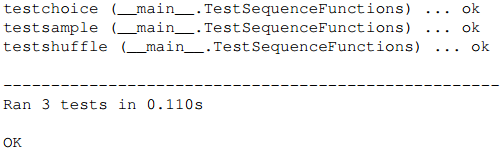
\includegraphics[scale=0.8]{images/tests.png}
        \end{center}
        \caption{xUnit output}
        \label{xUnit output}
      \end{figure}

        \subsubsection{Niveaux de tests}
        Le test peut être effectué à différents niveaux \ref{Testing levels}. Le plus bas niveau de test est appelé test unitaire. Une unité est la plus petite partie d’une application testable. Cela correspond une fonction ou une méthode dans une classe. Le but des tests unitaires est de vérifier que les différentes parties du code fonctionnent comme elles le devraient. Ils assurent la stabilité du code en testant chaque unité unitairement. Les régressions seront ainsi remontées très rapidement ce qui permet de manipuler le code source avec confiance. Les tests unitaires sont généralement écrits par le développeur qui a également écrit le code. Une bonne pratique des tests unitaires est de commencer par écrire les tests et d’ensuite les valider par le code. C’est ce qu’on appelle le « Tests Driven Development » (TDD) ou Développement Dirigé par les Tests ».\\

        Le niveau suivant est le test d'intégration. Dans ce contexte d’Intégration nous devons vérifier que les modules individuels du logiciel fonctionnent aussi en tant que groupe.\\

        \begin{quotation}
          \emph{« Le test d'intégration identifie les problèmes qui se produisent lors de la combinaison d'unités. En utilisant un plan de test exigeant que vous testiez chaque unité et que vous vérifiez la viabilité de chacune d'elles avant de les combiner, vous savez que les erreurs découvertes lors de la combinaison d'unités concernent probablement l'interface entre les unités. Cette méthode réduit le nombre de possibilités à un niveau beaucoup plus simple d'analyse. »} Microsoft \cite{Mic16}\\
        \end{quotation}

        Le troisième niveau teste les API d’un point de vue externe, sans se préoccuper de fonctionnement interne du système. Le test système analyse le flux de retour de l’API en fonction de son flux d’entrée afin  de détecter les défauts à la fois dans les inter-assemblages mais également au sein du système dans son ensemble. Cette méthode est appelé « boîte noire ».\\

	       Le test fonctionnel est le quatrième niveau de test majeur. Il assure la stabilité de l’application en reproduisant le parcours d’un utilisateur sur le navigateur. Il teste le bon fonctionnement de l’application et remontent les régressions fonctionnelles.\\

         D’autres niveaux de test existent, tel que le test applicatif qui assure la sécurité et la compatibilité, le test d’IHM qui fiabilise l’ergonomie et la visibilité, le test de charge qui veille à la performance et à la robustesse de l’application...

         \begin{figure}
           \begin{center}
             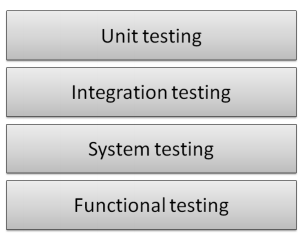
\includegraphics[scale=0.7]{images/testingLevels.png}
           \end{center}
           \caption{Les principaux niveaux de test}
           \label{Testing levels}
         \end{figure}

        \subsubsection{Exécuter les tests plus rapides en première}

        \subsubsection{Ecrire des tests d’échecs}

      \subsection{Base de données d’intégration}

      \subsection{Inspection Continue}

        \subsubsection{Différences entre inspection et test}

        \subsubsection{Rapport d’inspection}

    \section{Déploiement Continue}

      \subsection{Les bonnes pratiques du Déploiement Continue}

        \subsubsection{Etiqueter les actifs d’un référentiel}

        \subsubsection{Produire un environnement propre}

        \subsubsection{Etiqueter chaque build}

        \subsubsection{Exécuter tous les tests}

        \subsubsection{Créer des build feedback reports}

        \subsubsection{Capacité à effectuer un rollback}

      \subsection{La « bêta perpétuelle »}
      Le principe de la « bêta perpétuelle » a été introduit pour la première fois par Tim O’Reilly dans le manifeste du Web 2.0, qui expose le principe selon lequel:\\
      \begin{quotation}
        \emph{« Les utilisateurs doivent être considérés comme des co-développeurs, en suivant les principes Open Source (…). Avec le Web 2.0, ce principe évolue vers une position plus radicale, la bêta perpétuelle, dans laquelle le produit est développé de manière ouverte, avec de nouvelles fonctionnalités offertes sur une base mensuelle, hebdomadaire, ou même quotidienne. »}\\
      \end{quotation}

      Le terme « bêta perpétuelle » désigne le fait que notre application n’est jamais finalisée. Elle s’absout des contraintes habituelles liées au cycle de développement en « release » au profit d’une livraison en continu des nouvelles fonctionnalités.

        \subsubsection{Release early, release often}
        Derrière ce nouveau concept se cache un concept déjà bien en place chez les agilistes (du point de vue de l’itération courte) et dans le monde de l’Open Source (du point de vue de la récolte continue du feedback), le « Release early, release often », traduit en français par « Publiez tôt, publiez souvent ». Cette pratique a été décrite par Eric Steven Raymond dans “La cathédrale et le bazar” où il formulait explicitement:\\
        \begin{quotation}
          \emph{« Publiez tôt. Publiez souvent. Et écoutez vos clients »}\\
        \end{quotation}

        Cette méthodologie vise à réduire les temps de développement et améliorer l’implication de l’utilisateur dans la conception du logiciel afin de créer un produit correspondant à ces attentes et ainsi éviter la création d’un logiciel que personne n’utilisera.

        \subsubsection{Les services en ligne (Software As A Service)}
        Le concept de « bêta perpétuelle » a été rendu possible grâce au Cloud Computing et plus particulièrement à la généralisation du service en ligne ou « Software As A Service ». L’hébergement de l’application par l’éditeur permet d’absoudre ce dernier au traditionnel cycle de déploiement d’un logiciel et de ne gérer qu’une seule version de son application. Les services en ligne sont continuellement mise à jour sans pour autant en informer l’utilisateur. Les nouvelles fonctionnalités, découverte au fur et à mesure par l’utilisateur, permettent un apprentissage progressif des nouveautés applicatives.

        \subsubsection{La « Customer driven roadmap »}
        L’hébergement de l’application sur serveur offre à l’éditeur une maîtrise total de sa plateforme de production. Il peut ainsi mettre en place des sondes analytiques afin de récolter des informations sur l’usage de notre application et l’accueil réservé à nos nouvelles fonctionnalités par l’utilisateur.

        \subsubsection{Les pré-requis}
        La mise en place d’une stratégie de « bêta perpétuelle » requiert certains pré-requis pour en garantir le succès:\\
        \begin{itemize}
          \item une intégration continu,
          \item une livraison continue,
          \item un déploiement continu,
          \item une stratégie de type « One click deployment / Rollback » pour une restauration rapide de l’application au dernier état stable.\\
        \end{itemize}

        \subsubsection{Conclusion}
        Le concept de la « bêta perpétuelle » est présent chez de nombreux géants du Web tel que Google, Facebook, Amazon, Twitter, Flickr… Peu en font mention dû à la mauvaise image du terme « bêta », qui pour la conscience collective, se réfère à un produit non fini et peu fiable. Prenons en exemple Gmail, la boite aux lettres mails développé par Google, qui jusqu’en 2009 intégrait la mention « bêta » dans son logo. De petites fonctionnalités unitaires sont fréquemment proposés aux utilisateurs. En fonction de leur niveau d’adoption Google les intègrent ou non à la version standard de son service.

      \subsection{Le « Zero downtime deployment »}

          \subsubsection{Les patterns}
          Blue/Green Deployment\\

          Canary Release\\

          Dark Launch\\

          \subsubsection{La mise en oeuvre}
          Load balancer\\

          Les sessions\\

          La modification du schéma de base de données\\

        \subsection{Le « Flipping feature »}

    \chapter{Etude de l'art}

      \section{Logiciel en développement}

      \section{Processus de développement logiciel}

        \subsection{Scrum dans l'AgilLab}

        \subsection{Comment l’Intégration Continue s’intègre-t-elle dans le processus de développement logiciel}

        \subsection{Les équipes de développement}

      \section{La sécurité à l'esprit}

    \chapter{Implémentation}

      \section{Choisir ses outils}

        \subsection{Scaling}

        \subsection{Le choix du serveur d’Intégration Continue}
          \subsubsection{Support du langage de programmation}

          \subsubsection{Support du Source Code Management}

          \subsubsection{Gestion des builds}

          \subsubsection{Sécurité}

          \subsubsection{Autres caractéristiques}

          \subsubsection{Extensibilité}

          \subsubsection{Installation et configuration}

          \subsubsection{Autres questions à examiner}

      \section{Logiciels et outils utilisés}

        \subsection{Serveur d’Intégration Continue}

        \subsection{Logiciel de gestion de configuration}

        \subsection{Outils de build}

        \subsection{Automatisation des tests et de la couverture de code}

        \subsection{Documentation Continue}

        \subsection{Déploiement Continue}

        \subsection{Feedback Continue}

      \section{Architecture}

        \subsection{Serveur d’Intégration Continue}

        \subsection{Logiciel de gestion de configuration}

        \subsection{Réseaux et déploiement}

      \section{Configuration}

        \subsection{« Build jobs »}

          \subsubsection{Découpage des jobs}

          \subsubsection{Etablir des relations}

        \subsection{Reporting}

      \section{Délivrables et artéfacts de build}

  \listoffigures                  % Liste les figures
  \bibliographystyle{alpha}       % les trois premières lettres du nom de l'auteur accolées aux deux derniers chiffres de l'année de parution
  \bibliography{MemoireM2}        % mon fichier de base de données s'appelle MemoireM2.bib
\end{document}
